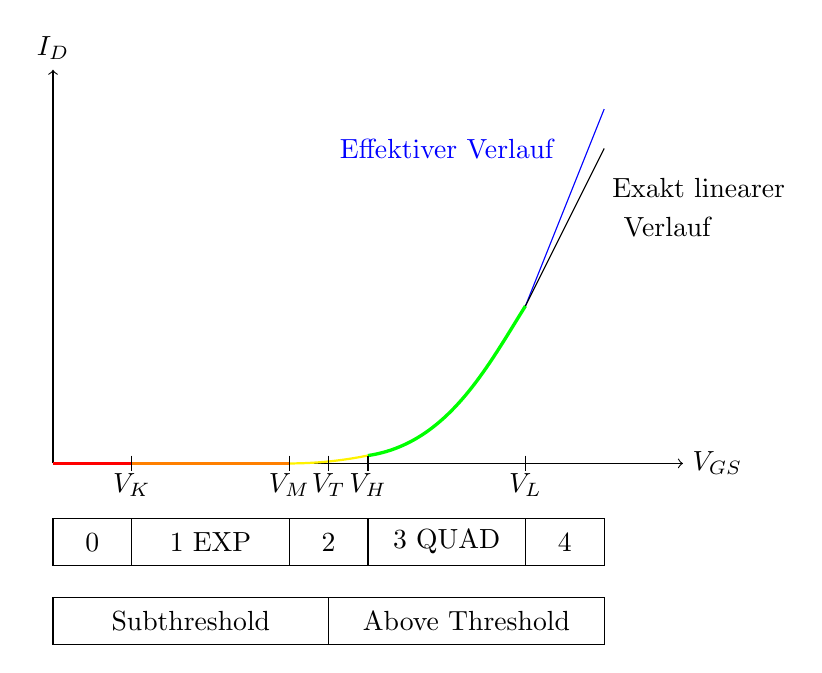
\begin{tikzpicture}

\draw [->] (0,0) -- (0,5) node [anchor=south] {$I_D$};
\draw [->] (0,0) -- (8,0) node [anchor=west] {$V_{GS}$};

\draw [color=red, thick] (0,0) -- (1,0);
\draw [color=orange, very thick] (1,0) -- (3,0);
\draw [color=yellow, thick] (3,0) arc (-90:-78:5);
\draw [color=green, very thick] (4.0,0.1) .. controls (5,0.25) and (5.5,1.2) .. (6,2);
\draw [color=blue] (6,2) -- (7,4.5);
\draw (6,2) -- (7,4);

\node [color=blue] at (5,4) {Effektiver Verlauf}; 
\node at (8.2,3.5) {Exakt linearer};
\node at (7.8,3) {Verlauf};


\foreach \x in {1,3,4,6} {
	\draw (\x,0.1) -- (\x,-0.1);
	\draw (\x,-0.7) -- (\x,-1.3);
}

\draw (3.5,0.1) -- (3.5,-0.1);

\draw (0,-0.7) rectangle (7,-1.3);

\node at (1,0) [anchor=north] {$V_K$};
\node at (3,0) [anchor=north] {$V_M$};
\node at (3.5,0) [anchor=north] {$V_T$};
\node at (4,0) [anchor=north] {$V_H$};
\node at (6,0) [anchor=north] {$V_L$};

\node at (0.5,-1) {0};
\node at (2,-1) {1 EXP};
\node at (3.5,-1) {2};
\node at (5,-1) {3 QUAD};
\node at (6.5,-1) {4};

\draw (0,-1.7) rectangle (7,-2.3);
\draw (3.5,-1.7) -- (3.5,-2.3);
\node at (1.75,-2) {Subthreshold};
\node at (3.5+1.75,-2) {Above Threshold};
\end{tikzpicture}